\documentclass{article}
\usepackage{amsmath, amssymb}
\usepackage{graphicx}
\usepackage{tikz}
\usetikzlibrary{arrows.meta, calc, positioning, angles, quotes}
\usepackage[margin=1in]{geometry}

% Font configuration for Kalpurush (Requires XeLaTeX or LuaLaTeX)
\usepackage{fontspec}
\setmainfont[Script=Bengali]{Kalpurush}

\begin{document}

\section*{ভেক্টর ও গতিবিদ্যার গাণিতিক সমস্যাবলি (Problem Set: Vectors \& Kinematics)}

% ----------------------------------------------------------------------
% Question 21
% ----------------------------------------------------------------------
\subsection*{প্রশ্ন ২১}
\textbf{প্রশ্ন:} একটি গতিশীল কণার অবস্থান ভেক্টর $\vec{r}(t) = (t^2 - 1)\hat{i} + 2t\hat{j}$ দ্বারা নির্দেশিত। কণাটির গতিপথের সমীকরণ প্রতিষ্ঠা করো এবং দেখাও যে, XY-সমতলে কণাটির সঞ্চারপথ একটি পরাবৃত্ত (parabola)। এই পরাবৃত্তের উপকেন্দ্র (focus) এবং নিয়ামকের (directrix) সমীকরণ নির্ণয় করো। 

[The position vector of a moving particle is given by $\vec{r}(t) = (t^2 - 1)\hat{i} + 2t\hat{j}$. Establish the equation of the trajectory of the particle and show that its locus in the XY-plane is a parabola. Find the focus and the equation of the directrix of this parabola.]

\begin{figure}[h!]
\centering
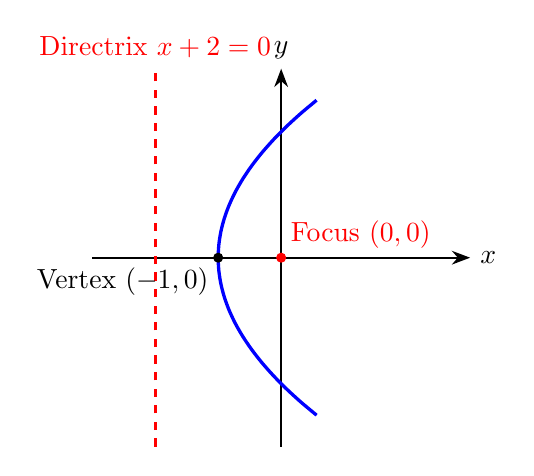
\begin{tikzpicture}[scale=0.8, >=Stealth]
    \draw[->, thick] (-3,0) -- (3,0) node[right] {$x$};
    \draw[->, thick] (0,-3) -- (0,3) node[above] {$y$};
    \draw[domain=-2.5:2.5, smooth, variable=\y, line width=1.2pt, blue] plot ({\y*\y/4 - 1}, {\y});
    \filldraw[red] (0,0) circle (2pt) node[above right] {Focus $(0,0)$};
    \draw[dashed, red, line width=1pt] (-2,-3) -- (-2,3) node[above] {Directrix $x+2=0$};
    \filldraw (-1,0) circle (2pt) node[below left] {Vertex $(-1,0)$};
\end{tikzpicture}
\caption{কণাটির গতিপথের পরাবৃত্তীয় রূপ (Parabolic trajectory of the particle)}
\end{figure}

\textbf{সমাধান:}

দেওয়া আছে, অবস্থান ভেক্টর $\vec{r}(t) = (t^2 - 1)\hat{i} + 2t\hat{j}$। কার্তেসীয় স্থানাঙ্ক অনুযায়ী পাই:

$$x = t^2 - 1 \quad \text{--- (i)}$$
$$y = 2t \implies t = \frac{y}{2} \quad \text{--- (ii)}$$

সমীকরণ (ii) থেকে $t$ এর মান সমীকরণ (i)-এ বসিয়ে পাই:

$$x = \left(\frac{y}{2}\right)^2 - 1 \implies x = \frac{y^2}{4} - 1$$
$$\Rightarrow y^2 = 4(x + 1)$$

এটি $y^2 = 4aX$ আকারের একটি আদর্শ পরাবৃত্তের সমীকরণ, যেখানে $X = x + 1$ এবং $a = 1$। যেহেতু সঞ্চারপথের সমীকরণটি এই আকারে প্রকাশ করা যায়, সেহেতু কণাটির গতিপথ একটি পরাবৃত্ত। (প্রমাণিত)

\textbf{উপকেন্দ্র (Focus) নির্ণয়:}

আদর্শ পরাবৃত্তের উপকেন্দ্রের স্থানাঙ্ক $(X, y) = (a, 0)$।

$$x + 1 = a \implies x + 1 = 1 \implies x = 0$$
$$y = 0$$

অতএব, পরাবৃত্তটির উপকেন্দ্র হলো মূলবিন্দু $(0, 0)$।

\textbf{নিয়ামকের (Directrix) সমীকরণ নির্ণয়:}

নিয়ামকের সমীকরণ $X = -a$:

$$x + 1 = -1 \implies x + 2 = 0$$

\textbf{উত্তর:} উপকেন্দ্র $(0, 0)$ এবং নিয়ামকের সমীকরণ $x + 2 = 0$

\hrulefill

% ----------------------------------------------------------------------
% Question 22
% ----------------------------------------------------------------------
\subsection*{প্রশ্ন ২২}
\textbf{প্রশ্ন:} $t = 0\text{ s}$ সময়ে একটি স্থির কণার উপর x-অক্ষ বরাবর $5\text{ m/s}^2$ ত্বরণ প্রয়োগ করা হলো। একই মুহূর্তে y-অক্ষের সাথে $30^\circ$ কোণে $3\text{ m/s}^2$ ত্বরণে বাতাস প্রবাহিত হওয়া শুরু হলো। $3\text{ s}$ পর কণাটির নিট সরণ এবং শেষ বেগ ভেক্টরের মান ও দিক নির্ণয় করো।

[At $t = 0\text{ s}$, an acceleration of $5\text{ m/s}^2$ along the x-axis is applied to a stationary particle. At the same moment, wind starts blowing with an acceleration of $3\text{ m/s}^2$ at an angle of $30^\circ$ with the y-axis. Determine the magnitude and direction of the net displacement and final velocity vectors of the particle after $3\text{ s}$.]

\begin{figure}[h!]
\centering
\begin{tikzpicture}[scale=1, >=Stealth]
    \draw[->, thick] (0,0) -- (4,0) node[right] {x-অক্ষ};
    \draw[->, thick] (0,0) -- (0,3) node[above] {y-অক্ষ};
    \draw[->, ultra thick, blue] (0,0) -- (3,0) node[below] {$\vec{a}_0 = 5\hat{i}$};
    \draw[->, ultra thick, green!50!black] (0,0) -- (1.299, 2.25) node[above right] {$\vec{a}_w = 3\text{ m/s}^2$};
    \draw[dashed] (0,1.5) arc (90:60:1.5);
    \node at (0.4, 1.8) {$30^\circ$};
    \draw[->, ultra thick, red] (0,0) -- (4.299, 2.25) node[right] {$\vec{a}_{net}$};
\end{tikzpicture}
\caption{ত্বরণ ভেক্টরের সংযোজন (Vector addition of accelerations)}
\end{figure}

\textbf{সমাধান:}

কণাটির উপর প্রযুক্ত আদি ত্বরণ $\vec{a}_0 = 5\hat{i}\text{ m/s}^2$। বাতাসের ত্বরণ $\vec{a}_w$ y-অক্ষের সাথে $30^\circ$ কোণে ক্রিয়াশীল হওয়ায় এর উপাংশসমূহ:

$$a_{wx} = 3\sin 30^\circ = 1.5\text{ m/s}^2$$
$$a_{wy} = 3\cos 30^\circ = 1.5\sqrt{3}\text{ m/s}^2$$

কণাটির লব্ধি ত্বরণ $\vec{a}$:

$$a_x = a_{0x} + a_{wx} = 5 + 1.5 = 6.5\text{ m/s}^2$$
$$a_y = a_{wy} = 1.5\sqrt{3}\text{ m/s}^2$$
$$\vec{a} = 6.5\hat{i} + 1.5\sqrt{3}\hat{j}\text{ m/s}^2$$

\textbf{সরণ ভেক্টর ($\vec{s}$) নির্ণয় (আদিবেগ $u = 0$):}

$$\vec{s} = \frac{1}{2}\vec{a}t^2 = \frac{1}{2}(6.5\hat{i} + 1.5\sqrt{3}\hat{j})(3)^2 = 4.5(6.5\hat{i} + 1.5\sqrt{3}\hat{j})$$
$$\vec{s} = 29.25\hat{i} + 6.75\sqrt{3}\hat{j}\text{ m} \approx 29.25\hat{i} + 11.69\hat{j}\text{ m}$$
$$s = \vert{}\vec{s}\vert{} = \sqrt{29.25^2 + (6.75\sqrt{3})^2} \approx \sqrt{855.56 + 136.69} \approx 31.50\text{ m}$$

\textbf{শেষ বেগ ভেক্টর ($\vec{v}$) নির্ণয়:}

$$\vec{v} = \vec{a}t = (6.5\hat{i} + 1.5\sqrt{3}\hat{j}) \times 3 = 19.5\hat{i} + 4.5\sqrt{3}\hat{j}\text{ m/s}$$
$$\vert{}\vec{v}\vert{} = \sqrt{19.5^2 + (4.5\sqrt{3})^2} = \sqrt{380.25 + 60.75} = \sqrt{441} = 21\text{ m/s}$$

\textbf{উত্তর:} নিট সরণ $31.50\text{ m}$ এবং শেষ বেগের মান $21\text{ m/s}$

\hrulefill

% ----------------------------------------------------------------------
% Question 23
% ----------------------------------------------------------------------
\subsection*{প্রশ্ন ২৩}
\textbf{প্রশ্ন:} একটি গাড়ি অনুভূমিকের সাথে $30^\circ$ কোণে আনত একটি পাহাড়ের ঢাল বরাবর $20\text{ m/s}$ বেগে উপরে উঠছে। ঠিক ওই সময়ে বৃষ্টি খাড়া নিচের দিকে $10\text{ m/s}$ বেগে পড়ছে এবং বাতাস পশ্চিম দিকে $5\text{ m/s}$ বেগে বইছে। গাড়িচালকের সাপেক্ষে বৃষ্টির আপেক্ষিক বেগ ভেক্টরটি নির্ণয় করো।

[A car is moving up an inclined hill slope at an angle of $30^\circ$ to the horizontal with a velocity of $20\text{ m/s}$. At that exact moment, rain is falling vertically downward at $10\text{ m/s}$ and wind is blowing westward at $5\text{ m/s}$. Find the relative velocity vector of the rain with respect to the driver of the car.]

\begin{figure}[h!]
\centering
\begin{tikzpicture}[scale=1, >=Stealth]
    \draw[thick] (0,0) -- (4,0);
    \draw[thick] (0,0) -- (3.46,2);
    \draw (0.8,0) arc (0:30:0.8);
    \node at (1.2,0.3) {$30^\circ$};
    
    \draw[->, ultra thick, blue] (1.73,1) -- ++(30:2) node[above left] {$\vec{v}_c = 20\text{ m/s}$};
    \draw[->, ultra thick, cyan] (2,3) -- (2,1) node[right] {বৃষ্টি ($10\text{ m/s}$)};
    \draw[->, ultra thick, gray] (2,3) -- (0.5,3) node[above] {বাতাস ($5\text{ m/s}$)};
\end{tikzpicture}
\caption{গাড়ি, বৃষ্টি ও বাতাসের বেগের দিক (Velocity vectors of car, rain, and wind)}
\end{figure}

\textbf{সমাধান:}

পূর্ব দিককে $+x$ অক্ষ ($\hat{i}$) এবং খাড়া উপরের দিককে $+y$ অক্ষ ($\hat{j}$) ধরি।

\textbf{গাড়ির বেগ ভেক্টর ($\vec{v}_c$):}

$$\vec{v}_c = 20\cos 30^\circ\hat{i} + 20\sin 30^\circ\hat{j} = 10\sqrt{3}\hat{i} + 10\hat{j}\text{ m/s}$$

\textbf{বৃষ্টির প্রকৃত বেগ ভেক্টর ($\vec{v}_{rain}$):}

$$\vec{v}_{rain} = -5\hat{i} - 10\hat{j}\text{ m/s}$$

\textbf{গাড়িচালকের সাপেক্ষে বৃষ্টির আপেক্ষিক বেগ ($\vec{v}_{rel}$):}

$$\vec{v}_{rel} = \vec{v}_{rain} - \vec{v}_c = (-5\hat{i} - 10\hat{j}) - (10\sqrt{3}\hat{i} + 10\hat{j})$$
$$\vec{v}_{rel} = -(5 + 10\sqrt{3})\hat{i} - 20\hat{j}\text{ m/s} \approx -22.32\hat{i} - 20\hat{j}\text{ m/s}$$

\textbf{উত্তর:} $-(5 + 10\sqrt{3})\hat{i} - 20\hat{j}\text{ m/s}$ (বা $-22.32\hat{i} - 20\hat{j}\text{ m/s}$)

\hrulefill

% ----------------------------------------------------------------------
% Question 24
% ----------------------------------------------------------------------
\subsection*{প্রশ্ন ২৪}
\textbf{প্রশ্ন:} ধরি $\vec{a} = \hat{i} + 2\hat{j} - \hat{k}$, $\vec{b} = \hat{i} - \hat{j}$ এবং $\vec{c} = \hat{i} - \hat{j} - \hat{k}$ তিনটি ভেক্টর। যদি $\vec{r}$ এমন একটি ভেক্টর হয় যা $\vec{r} \times \vec{a} = \vec{c} \times \vec{a}$ এবং $\vec{r} \cdot \vec{b} = 0$ সম্পর্ক দুটি সিদ্ধ করে, তবে $\vec{r} \cdot \vec{a}$ এর মান নির্ণয় করো।

[Let $\vec{a} = \hat{i} + 2\hat{j} - \hat{k}$, $\vec{b} = \hat{i} - \hat{j}$, and $\vec{c} = \hat{i} - \hat{j} - \hat{k}$ be three vectors. If $\vec{r}$ is a vector satisfying $\vec{r} \times \vec{a} = \vec{c} \times \vec{a}$ and $\vec{r} \cdot \vec{b} = 0$, find the value of $\vec{r} \cdot \vec{a}$.]

\begin{figure}[h!]
\centering
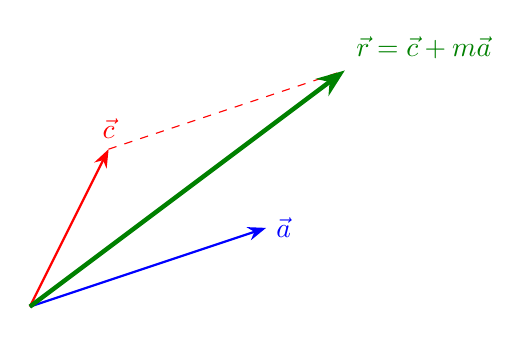
\begin{tikzpicture}[scale=1, >=Stealth]
    \draw[->, thick, blue] (0,0) -- (3,1) node[right] {$\vec{a}$};
    \draw[->, thick, red] (0,0) -- (1,2) node[above] {$\vec{c}$};
    \draw[dashed, red] (1,2) -- (4,3);
    \draw[->, ultra thick, green!50!black] (0,0) -- (4,3) node[above right] {$\vec{r} = \vec{c} + m\vec{a}$};
\end{tikzpicture}
\caption{ভেক্টর জ্যামিতিক উপস্থাপন (Geometric representation of vector $\vec{r}$)}
\end{figure}

\textbf{সমাধান:}

প্রথম সম্পর্কটি থেকে পাই:

$$\vec{r} \times \vec{a} = \vec{c} \times \vec{a} \implies (\vec{r} - \vec{c}) \times \vec{a} = \vec{0}$$

যেহেতু দুটি ভেক্টরের ক্রস গুণফল শূন্য, তাই $(\vec{r} - \vec{c})$ এবং $\vec{a}$ সমান্তরাল:

$$\vec{r} - \vec{c} = m\vec{a} \implies \vec{r} = \vec{c} + m\vec{a} \quad \text{--- (i)}$$

উভয় পক্ষে $\vec{b}$ দ্বারা ডট গুণ করি:

$$\vec{r} \cdot \vec{b} = \vec{c} \cdot \vec{b} + m(\vec{a} \cdot \vec{b})$$

শর্তানুসারে $\vec{r} \cdot \vec{b} = 0$:

$$0 = \vec{c} \cdot \vec{b} + m(\vec{a} \cdot \vec{b}) \quad \text{--- (ii)}$$

ভেক্টরগুলোর ডট গুণফল নির্ণয় করি:

$$\vec{a} \cdot \vec{b} = (1)(1) + (2)(-1) + (-1)(0) = -1$$
$$\vec{c} \cdot \vec{b} = (1)(1) + (-1)(-1) + (-1)(0) = 2$$

সমীকরণ (ii)-এ মান বসিয়ে পাই:

$$0 = 2 + m(-1) \implies m = 2$$

সুতরাং, $\vec{r} = \vec{c} + 2\vec{a}$।

এখন $\vec{r} \cdot \vec{a}$ নির্ণয় করি:

$$\vec{r} \cdot \vec{a} = (\vec{c} + 2\vec{a}) \cdot \vec{a} = \vec{c} \cdot \vec{a} + 2\vert{}\vec{a}\vert{}^2$$

এখানে:

$$\vec{c} \cdot \vec{a} = (1)(1) + (-1)(2) + (-1)(-1) = 0$$
$$\vert{}\vec{a}\vert{}^2 = 1^2 + 2^2 + (-1)^2 = 6$$
$$\vec{r} \cdot \vec{a} = 0 + 2(6) = 12$$

\textbf{উত্তর:} $12$

\hrulefill

% ----------------------------------------------------------------------
% Question 25
% ----------------------------------------------------------------------
\subsection*{প্রশ্ন ২৫}
\textbf{প্রশ্ন:} ত্রিমাত্রিক স্থানে দুটি ভেক্টর যথাক্রমে $\vec{a} = \frac{\hat{i} - 2\hat{j}}{\sqrt{5}}$ এবং $\vec{b} = \frac{2\hat{i} + \hat{j} + 3\hat{k}}{\sqrt{14}}$ দ্বারা সংজ্ঞায়িত। স্কেলার রাশি $(2\vec{a} + \vec{b}) \cdot [(\vec{a} \times \vec{b}) \times (\vec{a} - 2\vec{b})]$ এর মান নির্ণয় করো।

[In 3D space, two vectors are defined as $\vec{a} = \frac{\hat{i} - 2\hat{j}}{\sqrt{5}}$ and $\vec{b} = \frac{2\hat{i} + \hat{j} + 3\hat{k}}{\sqrt{14}}$. Find the value of the scalar quantity $(2\vec{a} + \vec{b}) \cdot [(\vec{a} \times \vec{b}) \times (\vec{a} - 2\vec{b})]$.]

\begin{figure}[h!]
\centering
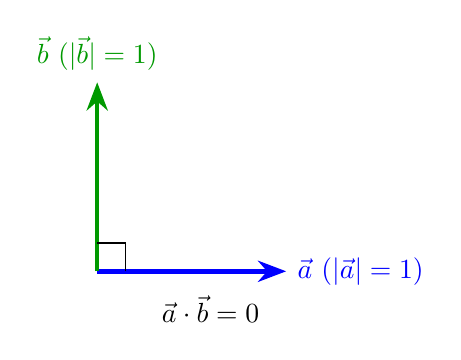
\begin{tikzpicture}[scale=1.2, >=Stealth]
    \draw[->, ultra thick, blue] (0,0) -- (2,0) node[right] {$\vec{a}$ ($|\vec{a}|=1$)};
    \draw[->, ultra thick, green!60!black] (0,0) -- (0,2) node[above] {$\vec{b}$ ($|\vec{b}|=1$)};
    \draw (0.3,0) -- (0.3,0.3) -- (0,0.3);
    \node at (1.2,-0.4) {$\vec{a} \cdot \vec{b} = 0$};
\end{tikzpicture}
\caption{পরস্পর লম্ব একক ভেক্টরদ্বয় (Orthogonal unit vectors $\vec{a}$ and $\vec{b}$)}
\end{figure}

\textbf{সমাধান:}

ভেক্টরদ্বয়ের মান ও ডট গুণফল:

$$\vert{}\vec{a}\vert{} = \frac{\sqrt{1^2 + (-2)^2}}{\sqrt{5}} = 1, \quad \vert{}\vec{b}\vert{} = \frac{\sqrt{2^2 + 1^2 + 3^2}}{\sqrt{14}} = 1$$
$$\vec{a} \cdot \vec{b} = \frac{1(2) + (-2)(1) + 0(3)}{\sqrt{70}} = 0$$

অর্থাৎ, $\vec{a}$ ও $\vec{b}$ দুটি লম্ব একক ভেক্টর।

ভেক্টর ত্রয়ী গুণফলের সূত্র $(\vec{x} \times \vec{y}) \times \vec{z} = (\vec{x} \cdot \vec{z})\vec{y} - (\vec{y} \cdot \vec{z})\vec{x}$ প্রয়োগ করে পাই:

$$(\vec{a} \times \vec{b}) \times (\vec{a} - 2\vec{b}) = [\vec{a} \cdot (\vec{a} - 2\vec{b})]\vec{b} - [\vec{b} \cdot (\vec{a} - 2\vec{b})]\vec{a}$$
$$= [\vec{a} \cdot \vec{a} - 2(\vec{a} \cdot \vec{b})]\vec{b} - [\vec{b} \cdot \vec{a} - 2(\vec{b} \cdot \vec{b})]\vec{a}$$
$$= (1 - 0)\vec{b} - (0 - 2)\vec{a} = 2\vec{a} + \vec{b}$$

মূল রাশিতে এটি বসিয়ে পাই:

$$(2\vec{a} + \vec{b}) \cdot (2\vec{a} + \vec{b}) = 4\vert{}\vec{a}\vert{}^2 + \vert{}\vec{b}\vert{}^2 + 4(\vec{a} \cdot \vec{b}) = 4(1) + 1 + 0 = 5$$

\textbf{উত্তর:} $5$

\hrulefill

% ----------------------------------------------------------------------
% Question 26
% ----------------------------------------------------------------------
\subsection*{প্রশ্ন ২৬}
\textbf{প্রশ্ন:} যদি $\vec{a}, \vec{b}$ এবং $\vec{c}$ তিনটি একক ভেক্টর হয় যারা $\vert{}\vec{a} - \vec{b}\vert{}^2 + \vert{}\vec{b} - \vec{c}\vert{}^2 + \vert{}\vec{c} - \vec{a}\vert{}^2 = 9$ সমীকরণটি সিদ্ধ করে, তবে $\vert{}2\vec{a} + 5\vec{b} + 5\vec{c}\vert{}$ এর মান নির্ণয় করো।

[If $\vec{a}, \vec{b}$, and $\vec{c}$ are three unit vectors satisfying $\vert{}\vec{a} - \vec{b}\vert{}^2 + \vert{}\vec{b} - \vec{c}\vert{}^2 + \vert{}\vec{c} - \vec{a}\vert{}^2 = 9$, find the value of $\vert{}2\vec{a} + 5\vec{b} + 5\vec{c}\vert{}$.]

\begin{figure}[h!]
\centering
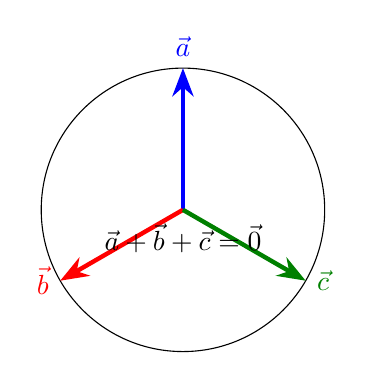
\begin{tikzpicture}[scale=1.2, >=Stealth]
    \draw (0,0) circle (1.5cm);
    \draw[->, ultra thick, blue] (0,0) -- (90:1.5) node[above] {$\vec{a}$};
    \draw[->, ultra thick, red] (0,0) -- (210:1.5) node[left] {$\vec{b}$};
    \draw[->, ultra thick, green!50!black] (0,0) -- (330:1.5) node[right] {$\vec{c}$};
    \node at (0,-0.3) {$\vec{a}+\vec{b}+\vec{c}=\vec{0}$};
\end{tikzpicture}
\caption{সাম্যাবস্থায় তিনটি একক ভেক্টর (Equilibrium of three unit vectors)}
\end{figure}

\textbf{সমাধান:}

যেহেতু $\vec{a}, \vec{b}, \vec{c}$ একক ভেক্টর, তাই $\vert{}\vec{a}\vert{} = \vert{}\vec{b}\vert{} = \vert{}\vec{c}\vert{} = 1$।

$$\vert{}\vec{a} - \vec{b}\vert{}^2 = \vert{}\vec{a}\vert{}^2 + \vert{}\vec{b}\vert{}^2 - 2\vec{a} \cdot \vec{b} = 2 - 2\vec{a} \cdot \vec{b}$$

একইভাবে প্রদত্ত সমীকরণ সম্প্রসারণ করে পাই:

$$(2 - 2\vec{a} \cdot \vec{b}) + (2 - 2\vec{b} \cdot \vec{c}) + (2 - 2\vec{c} \cdot \vec{a}) = 9$$
$$\Rightarrow 6 - 2(\vec{a} \cdot \vec{b} + \vec{b} \cdot \vec{c} + \vec{c} \cdot \vec{a}) = 9 \implies \vec{a} \cdot \vec{b} + \vec{b} \cdot \vec{c} + \vec{c} \cdot \vec{a} = -\frac{3}{2}$$

এখন, $\vert{}\vec{a} + \vec{b} + \vec{c}\vert{}^2$ এর বিস্তার করি:

$$\vert{}\vec{a} + \vec{b} + \vec{c}\vert{}^2 = 1 + 1 + 1 + 2\left(-\frac{3}{2}\right) = 3 - 3 = 0$$
$$\Rightarrow \vec{a} + \vec{b} + \vec{c} = \vec{0} \implies \vec{b} + \vec{c} = -\vec{a}$$

কাঙ্খিত মান:

$$\vert{}2\vec{a} + 5\vec{b} + 5\vec{c}\vert{} = \vert{}2\vec{a} + 5(\vec{b} + \vec{c})\vert{} = \vert{}2\vec{a} - 5\vec{a}\vert{} = \vert{}-3\vec{a}\vert{} = 3\vert{}\vec{a}\vert{} = 3$$

\textbf{উত্তর:} $3$

\hrulefill

% ----------------------------------------------------------------------
% Question 27
% ----------------------------------------------------------------------
\subsection*{প্রশ্ন ২৭}
\textbf{প্রশ্ন:} একই সরলরেখা বরাবর একই অভিমুখে দুটি গাড়ি $30\text{ km/h}$ গতিতে চলছে এবং তাদের মধ্যবর্তী দূরত্ব $5\text{ km}$। বিপরীত দিক থেকে আসা একটি তৃতীয় গাড়ি পরপর দুটি গাড়ির সাথে $4\text{ min}$ সময়ের ব্যবধানে মিলিত হয়। তৃতীয় গাড়িটির প্রকৃত বেগের মান নির্ণয় করো।

[Two cars are moving in the same direction along the same straight line with a speed of $30\text{ km/h}$, separated by a distance of $5\text{ km}$. A third car coming from the opposite direction meets the two cars at a time interval of $4\text{ min}$. Determine the magnitude of the actual velocity of the third car.]

\begin{figure}[h!]
\centering
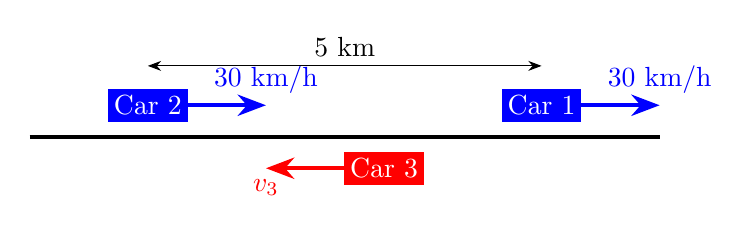
\begin{tikzpicture}[scale=1, >=Stealth]
    \draw[line width=1.5pt] (-1,0) -- (7,0);
    \filldraw[blue] (0,0.2) rectangle (1,0.6) node[midway, white] {Car 2};
    \filldraw[blue] (5,0.2) rectangle (6,0.6) node[midway, white] {Car 1};
    \filldraw[red] (3,-0.6) rectangle (4,-0.2) node[midway, white] {Car 3};
    
    \draw[->, ultra thick, blue] (1,0.4) -- (2,0.4) node[above] {$30\text{ km/h}$};
    \draw[->, ultra thick, blue] (6,0.4) -- (7,0.4) node[above] {$30\text{ km/h}$};
    \draw[->, ultra thick, red] (3,-0.4) -- (2,-0.4) node[below] {$v_3$};
    
    \draw[<->] (0.5, 0.9) -- (5.5, 0.9) node[midway, above] {$5\text{ km}$};
\end{tikzpicture}
\caption{গাড়ি তিনটির গতির চিত্র (Relative motion of the three cars)}
\end{figure}

\textbf{সমাধান:}

ধরি প্রথম দুটি গাড়ির বেগ $v_1 = v_2 = 30\text{ km/h}$ এবং ৩য় গাড়ির প্রকৃত বেগ $v_3$।

বিপরীত অভিমুখে গতিশীল হওয়ায় ১ম ও ২য় গাড়ির সাপেক্ষে ৩য় গাড়ির আপেক্ষিক বেগ:

$$v_{rel} = v_3 + 30\text{ km/h}$$

দেওয়া আছে, $d = 5\text{ km}$ এবং সময় $t = 4\text{ min} = \frac{4}{60}\text{ h} = \frac{1}{15}\text{ h}$।

আপেক্ষিক গতিবেগের সূত্রানুসারে:

$$d = v_{rel} \times t \implies 5 = (v_3 + 30) \times \frac{1}{15}$$
$$\Rightarrow v_3 + 30 = 75 \implies v_3 = 45\text{ km/h}$$

\textbf{উত্তর:} $45\text{ km/h}$

\hrulefill

% ----------------------------------------------------------------------
% Question 28
% ----------------------------------------------------------------------
\subsection*{প্রশ্ন ২৮}
\textbf{প্রশ্ন:} যদি $\vec{A} = \hat{i} - \hat{j} + 2\hat{k}$ হয় এবং $\vec{B}$ এমন একটি ভেক্টর হয় যা $\vec{A} \times \vec{B} = 2\hat{i} - \hat{k}$ এবং $\vec{A} \cdot \vec{B} = 3$ সম্পর্ক দুটি সিদ্ধ করে, তবে $\vec{A} - \vec{B}$ ভেক্টর বরাবর $\vec{B}$ ভেক্টরের লম্ব অভিক্ষেপ (projection) নির্ণয় করো।

[If $\vec{A} = \hat{i} - \hat{j} + 2\hat{k}$ and $\vec{B}$ is a vector satisfying $\vec{A} \times \vec{B} = 2\hat{i} - \hat{k}$ and $\vec{A} \cdot \vec{B} = 3$, find the projection of vector $\vec{B}$ along vector $\vec{A} - \vec{B}$.]

\begin{figure}[h!]
\centering
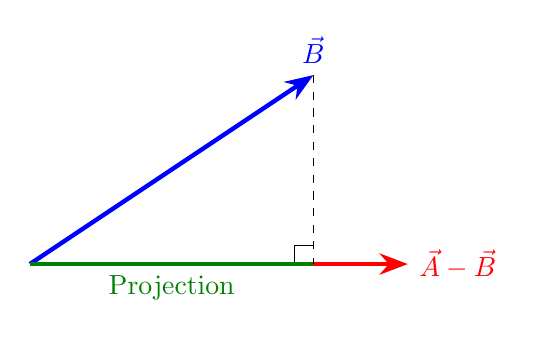
\begin{tikzpicture}[scale=1.2, >=Stealth]
    \draw[->, ultra thick, blue] (0,0) -- (3,2) node[above] {$\vec{B}$};
    \draw[->, ultra thick, red] (0,0) -- (4,0) node[right] {$\vec{A} - \vec{B}$};
    \draw[dashed] (3,2) -- (3,0);
    \draw (2.8,0) -- (2.8,0.2) -- (3,0.2);
    \draw[ultra thick, green!50!black] (0,0) -- (3,0) node[midway, below] {Projection};
\end{tikzpicture}
\caption{লম্ব অভিক্ষেপ (Vector Projection of $\vec{B}$ on $\vec{A}-\vec{B}$)}
\end{figure}

\textbf{সমাধান:}

ল্যাগরেঞ্জের অভেদ ($\vert{}\vec{A} \times \vec{B}\vert{}^2 + (\vec{A} \cdot \vec{B})^2 = \vert{}\vec{A}\vert{}^2 \vert{}\vec{B}\vert{}^2$) ব্যবহার করে পাই:

$$\vert{}\vec{A}\vert{}^2 = 1^2 + (-1)^2 + 2^2 = 6$$
$$\vert{}\vec{A} \times \vec{B}\vert{}^2 = 2^2 + (-1)^2 = 5$$
$$5 + 3^2 = 6\vert{}\vec{B}\vert{}^2 \implies 14 = 6\vert{}\vec{B}\vert{}^2 \implies \vert{}\vec{B}\vert{}^2 = \frac{7}{3}$$

$\vec{A} - \vec{B}$ বরাবর $\vec{B}$ এর লম্ব অভিক্ষেপ:

$$\text{Projection} = \frac{\vec{B} \cdot (\vec{A} - \vec{B})}{\vert{}\vec{A} - \vec{B}\vert{}} = \frac{\vec{A} \cdot \vec{B} - \vert{}\vec{B}\vert{}^2}{\sqrt{\vert{}\vec{A} - \vec{B}\vert{}^2}}$$

হর (denominator) হিসাব করি:

$$\vert{}\vec{A} - \vec{B}\vert{}^2 = \vert{}\vec{A}\vert{}^2 + \vert{}\vec{B}\vert{}^2 - 2(\vec{A} \cdot \vec{B}) = 6 + \frac{7}{3} - 6 = \frac{7}{3}$$
$$\implies \vert{}\vec{A} - \vec{B}\vert{} = \sqrt{\frac{7}{3}}$$

লব (numerator) হিসাব করি:

$$\vec{A} \cdot \vec{B} - \vert{}\vec{B}\vert{}^2 = 3 - \frac{7}{3} = \frac{2}{3}$$

অতএব, লম্ব অভিক্ষেপ:

$$\text{Projection} = \frac{\frac{2}{3}}{\sqrt{\frac{7}{3}}} = \frac{2}{\sqrt{21}}$$

\textbf{উত্তর:} $\frac{2}{\sqrt{21}}$ (বা $\approx 0.436$)

\hrulefill

% ----------------------------------------------------------------------
% Question 29
% ----------------------------------------------------------------------
\subsection*{প্রশ্ন ২৯}
\textbf{প্রশ্ন:} যদি $\vec{a}$, $\vec{b}$ এবং $\vec{c}$ তিনটি অশূন্য এবং অসমতলীয় ভেক্টর হয় এবং অপর তিনটি ভেক্টর যথাক্রমে $\vec{p} = \vec{a} + \vec{b} - 2\vec{c}$, $\vec{q} = 3\vec{a} - 2\vec{b} + \vec{c}$ এবং $\vec{r} = \vec{a} - 4\vec{b} + 2\vec{c}$ হয়, তবে $\vec{a}, \vec{b}, \vec{c}$ দ্বারা গঠিত সামান্তরিকীয় ঘনকের আয়তন $V_1$ এবং $\vec{p}, \vec{q}, \vec{r}$ দ্বারা গঠিত সামান্তরিকীয় ঘনকের আয়তন $V_2$ হলে, $\frac{V_2}{V_1}$ এর অনুপাত নির্ণয় করো।

[If $\vec{a}$, $\vec{b}$, and $\vec{c}$ are three non-zero non-coplanar vectors, and three other vectors are $\vec{p} = \vec{a} + \vec{b} - 2\vec{c}$, $\vec{q} = 3\vec{a} - 2\vec{b} + \vec{c}$, and $\vec{r} = \vec{a} - 4\vec{b} + 2\vec{c}$, find the ratio $\frac{V_2}{V_1}$, where $V_1$ is the volume of the parallelepiped formed by $\vec{a}, \vec{b}, \vec{c}$ and $V_2$ is the volume of the parallelepiped formed by $\vec{p}, \vec{q}, \vec{r}$.]

\begin{figure}[h!]
\centering
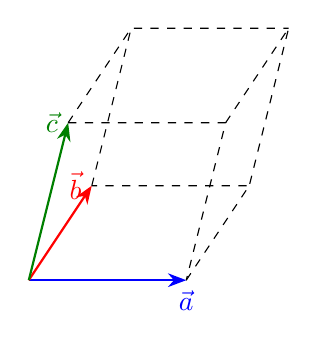
\begin{tikzpicture}[scale=1, >=Stealth]
    \draw[->, thick, blue] (0,0) -- (2,0) node[below] {$\vec{a}$};
    \draw[->, thick, red] (0,0) -- (0.8,1.2) node[left] {$\vec{b}$};
    \draw[->, thick, green!50!black] (0,0) -- (0.5,2) node[left] {$\vec{c}$};
    
    \draw[dashed] (2,0) -- (2.8,1.2) -- (0.8,1.2);
    \draw[dashed] (0.5,2) -- (2.5,2) -- (2,0);
    \draw[dashed] (2.5,2) -- (3.3,3.2) -- (2.8,1.2);
    \draw[dashed] (0.5,2) -- (1.3,3.2) -- (3.3,3.2);
    \draw[dashed] (0.8,1.2) -- (1.3,3.2);
\end{tikzpicture}
\caption{সামান্তরিকীয় ঘনক (Parallelepiped formed by vectors)}
\end{figure}

\textbf{সমাধান:}

প্রথম ঘনকের আয়তন $V_1 = \vert{}[\vec{a} \ \vec{b} \ \vec{c}]\vert{}$ এবং দ্বিতীয় ঘনকের আয়তন $V_2 = \vert{}[\vec{p} \ \vec{q} \ \vec{r}]\vert{}$।

ভেক্টরগুলোর সহগ দিয়ে গঠিত ম্যাট্রিক্স $M$:

$$M = \begin{pmatrix} 1 & 1 & -2 \\ 3 & -2 & 1 \\ 1 & -4 & 2 \end{pmatrix}$$

স্কেলার ত্রয়ী গুণফলের বৈশিষ্ট্যানুসারে $[\vec{p} \ \vec{q} \ \vec{r}] = \det(M) \cdot [\vec{a} \ \vec{b} \ \vec{c}]$।

$\det(M)$ এর মান নির্ণয় করি:

$$\det(M) = 1[(-2)(2) - (1)(-4)] - 1[(3)(2) - (1)(1)] - 2[(3)(-4) - (-2)(1)]$$
$$\Rightarrow \det(M) = 1(0) - 1(5) - 2(-10) = -5 + 20 = 15$$

অতএব, $V_2 = 15 V_1 \implies \frac{V_2}{V_1} = 15$।

\textbf{উত্তর:} $15$

\hrulefill

% ----------------------------------------------------------------------
% Question 30
% ----------------------------------------------------------------------
\subsection*{প্রশ্ন ৩০}
\textbf{প্রশ্ন:} যদি তিনটি অশূন্য ভেক্টর $\vec{a}$, $\vec{b}$ এবং $\vec{c}$ এর জন্য $(\vec{a} \times \vec{b}) \times \vec{c} = \vec{a} \times (\vec{b} \times \vec{c})$ সম্পর্কটি সত্য হয়, যেখানে $\vec{a} \cdot \vec{b} \neq 0$ এবং $\vec{b} \cdot \vec{c} \neq 0$। ভেক্টর বীজগণিতের সূত্রাবলি ব্যবহার করে প্রমাণ করো যে, $\vec{a}$ এবং $\vec{c}$ ভেক্টরদ্বয় পরস্পর সমান্তরাল।

[If for three non-zero vectors $\vec{a}$, $\vec{b}$, and $\vec{c}$, the relation $(\vec{a} \times \vec{b}) \times \vec{c} = \vec{a} \times (\vec{b} \times \vec{c})$ holds true, where $\vec{a} \cdot \vec{b} \neq 0$ and $\vec{b} \cdot \vec{c} \neq 0$, prove using vector algebra that the vectors $\vec{a}$ and $\vec{c}$ are parallel to each other.]

\begin{figure}[h!]
\centering
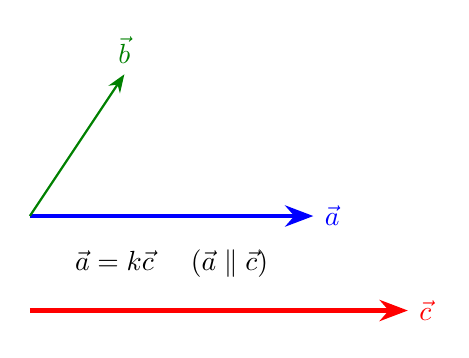
\begin{tikzpicture}[scale=1.2, >=Stealth]
    \draw[->, ultra thick, blue] (0,0.5) -- (3,0.5) node[right] {$\vec{a}$};
    \draw[->, ultra thick, red] (0,-0.5) -- (4,-0.5) node[right] {$\vec{c}$};
    \draw[->, thick, green!50!black] (0,0.5) -- (1,2) node[above] {$\vec{b}$};
    \node at (1.5, 0) {$\vec{a} = k\vec{c}$ \quad ($\vec{a} \parallel \vec{c}$)};
\end{tikzpicture}
\caption{পরস্পর সমান্তরাল ভেক্টরদ্বয় $\vec{a}$ ও $\vec{c}$ (Parallel vectors $\vec{a}$ and $\vec{c}$)}
\end{figure}

\textbf{সমাধান:}

ভেক্টর ত্রয়ী গুণফলের সূত্রানুসারে:

$$\text{LHS: } (\vec{a} \times \vec{b}) \times \vec{c} = (\vec{a} \cdot \vec{c})\vec{b} - (\vec{b} \cdot \vec{c})\vec{a}$$
$$\text{RHS: } \vec{a} \times (\vec{b} \times \vec{c}) = (\vec{a} \cdot \vec{c})\vec{b} - (\vec{a} \cdot \vec{b})\vec{c}$$

প্রদত্ত শর্তানুসারে $\text{LHS} = \text{RHS}$:

$$(\vec{a} \cdot \vec{c})\vec{b} - (\vec{b} \cdot \vec{c})\vec{a} = (\vec{a} \cdot \vec{c})\vec{b} - (\vec{a} \cdot \vec{b})\vec{c}$$

উভয় পক্ষ থেকে $(\vec{a} \cdot \vec{c})\vec{b}$ বাদ দিলে পাই:

$$-(\vec{b} \cdot \vec{c})\vec{a} = -(\vec{a} \cdot \vec{b})\vec{c} \implies \vec{a} = \left(\frac{\vec{a} \cdot \vec{b}}{\vec{b} \cdot \vec{c}}\right)\vec{c}$$

ধরি, $k = \frac{\vec{a} \cdot \vec{b}}{\vec{b} \cdot \vec{c}}$ একটি স্কেলার ধ্রুবক।

$$\vec{a} = k\vec{c}$$

যেহেতু একটি ভেক্টরকে অন্যটির স্কেলার গুণিতক হিসেবে প্রকাশ করা গেছে, সেহেতু $\vec{a}$ এবং $\vec{c}$ ভেক্টরদ্বয় পরস্পরের সমান্তরাল। (প্রমাণিত)

\end{document}